% Q18：按原图关键点恢复的一个周期；横坐标以 pi/2 为单位标注。
% 原图特征：零点 -pi/2、3pi/2、7pi/2；最大值 (pi/2,2)；最小值 (5pi/2,-2)。
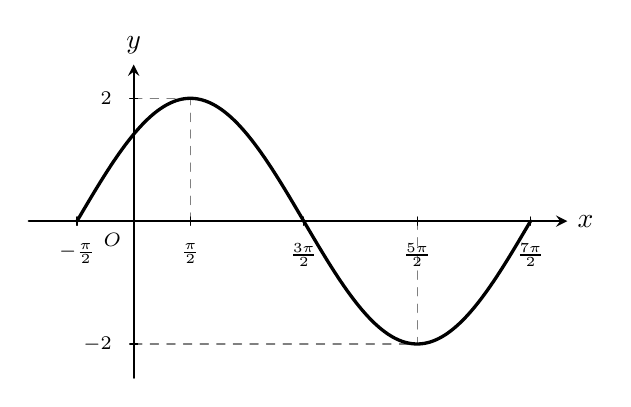
\begin{tikzpicture}[x=0.72cm,y=0.78cm,line cap=round,line join=round,>=stealth]
  \draw[->,thick] (-1.85,0)--(7.65,0) node[right] {$x$};
  \draw[->,thick] (0,-2.55)--(0,2.55) node[above] {$y$};

  \draw[dashed,gray] (0,2)--(1,2);
  \draw[dashed,gray] (1,0)--(1,2);
  \draw[dashed,gray] (0,-2)--(5,-2);
  \draw[dashed,gray] (5,0)--(5,-2);

  \draw[very thick] plot[domain=-90:630,samples=181] ({\x/90},{2*sin(\x/2+45)});

  \foreach \x/\label in {
    -1/{-\frac{\pi}{2}},
    1/{\frac{\pi}{2}},
    3/{\frac{3\pi}{2}},
    5/{\frac{5\pi}{2}},
    7/{\frac{7\pi}{2}}
  } {
    \draw (\x,0.07)--(\x,-0.07) node[below=3pt,font=\scriptsize] {$\label$};
  }
  \draw (0.07,2)--(-0.07,2) node[left=3pt,font=\scriptsize] {$2$};
  \draw (0.07,-2)--(-0.07,-2) node[left=3pt,font=\scriptsize] {$-2$};
  \node[below left=1pt,font=\scriptsize] at (0,0) {$O$};
\end{tikzpicture}
